% -*- root: ../../main.tex -*- %

\AnhChapter{Theoretical Background}
  \AnhSection{Docker}
    \begin{figure}[htbp]
      \centering
      \begin{tikzpicture}[scale=0.8,->,>=stealth',shorten >=1pt,auto,node distance=5cm, semithick]
        \sffamily\fontsize{10}{10}\selectfont
        \node (cr){};
        \node (run){};
        \node[state] (A)     [right =3cm of cr]         {created};
        \node[state]         (B) [right =2.5cm of A] {running};
        \node[state]         (C) [below right of=B] {stopped};
        \node[state]         (D) [above =2cm of B] {paused};
        \node[state]         (E) [below =2cm of A] {deleted};

        \path (cr) edge [] node {create} (A)
            (run) edge [out=45,in=150]                     node {run} (B)
              (A) edge []                              node {start} (B)
                  edge [bend right]                    node {rm}    (E)
              (B) edge [out=230, in=200, distance=4cm] node {kill}  (C)
                  edge [out=250,in=175, distance=2.5cm]node {stop}  (C)
                  edge [bend left]                     node {pause}  (D)
                  edge [in=30, out=45, loop]           node {restart}  (D)
                  edge [out=10, in=90, distance=2cm]   node {\textit{container process exited}}  (C)
              (C) edge [bend right]                    node {start}  (B)
                  edge [bend left]                     node {rm}  (E)
              (D) edge [bend left]                     node {unpause} (B)
              ;
      \end{tikzpicture}
      \caption*{Simplified version. Commands should be understood prefixed with \texttt{docker}. \newline \scriptsize Based on https://docs.docker.com/engine/reference/api/docker\_remote\_api/\#docker-events }
      \caption[Docker Container Life Cycle]{Docker Container Life Cycle \cite{Docker2016Docker}}
      \label{fig:docker_container_lifecycle}
    \end{figure}

\AnhChapter{Architecture and design}

  \begin{figure}[htbp]
    \centering
    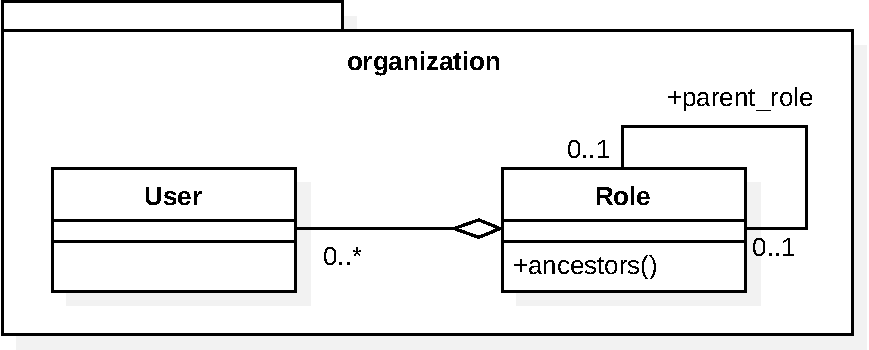
\includegraphics[width=0.65\textwidth]{content/images/class_diagram_organization-crop.pdf}
    \caption{UML Class Diagram for the Organization Service}
  \label{fig:uml_class_diagram_organization}
  \end{figure}

 \clearpage
\AnhChapter{Implementation}
  \AnhSection{Workflow image}

    \begin{listing}[!h]
      \inputminted[fontsize=\footnotesize,linenos=true,numberblanklines=true,showspaces=false,breaklines=true,baselinestretch=1]{json}{./content/snippets/process_definition.json}
      \caption{Exported process definition in JSON format}
    \label{lst:exported_process_definition_in_json_format}
    \end{listing}

    \begin{listing}[!h]
      \inputminted[fontsize=\footnotesize,linenos=true,numberblanklines=true,showspaces=false,breaklines=true,baselinestretch=1]{json}{./content/snippets/wf_image/input.schema.json}
      \caption*{ \mintinline{json}| {"this":"is a test"} | would be considered valid input data with the depicted schema }
      \caption{JSON schema used for input validation}
    \label{lst:input_schema_in_json_format}
    \end{listing}

    \begin{listing}[!h]
      \inputminted[fontsize=\footnotesize,linenos=true,numberblanklines=true,showspaces=false,breaklines=true,baselinestretch=1]{Dockerfile}{../code/wf_base/Dockerfile}
      \caption{Dockerfile for workflow base image}
    \label{lst:dockerfile_for_workflow_base_image}
    \end{listing}

    \begin{listing}[!h]
      \inputminted[lastline=39,fontsize=\footnotesize,linenos=true,numberblanklines=true,showspaces=false,breaklines=true,baselinestretch=1]{ruby}{../code/wf_base/activity_instance.rb}
      \caption{ActivityInstance class in workflow image (1/2)}
    \label{lst:wf_image_activity_instance}
    \end{listing}

    \begin{listing}[!h]
      \inputminted[firstline=40,fontsize=\footnotesize,linenos=true,numberblanklines=true,showspaces=false,breaklines=true,baselinestretch=1]{ruby}{../code/wf_base/activity_instance.rb}
      \caption{ActivityInstance class in workflow image (2/2)}
    \label{lst:wf_image_activity_instance_2}
    \end{listing}

    \begin{listing}[!h]
      \inputminted[fontsize=\footnotesize,linenos=true,numberblanklines=true,showspaces=false,breaklines=true,baselinestretch=1]{ruby}{../code/wf_base/file_helper.rb}
      \caption{FileHelper helper class in workflow image}
    \label{lst:wf_image_file_helper}
    \end{listing}
    ** overflow

    \begin{listing}[!h]
      \inputminted[fontsize=\footnotesize,linenos=true,numberblanklines=true,showspaces=false,breaklines=true,baselinestretch=1]{ruby}{../code/wf_base/process_definition.rb}
      \caption{ProcessDefinition class in workflow image}
    \label{lst:wf_image_process_definition}
    \end{listing}

    \begin{listing}[!h]
      \inputminted[lastline=45,fontsize=\footnotesize,linenos=true,numberblanklines=true,showspaces=false,breaklines=true,baselinestretch=1]{ruby}{../code/wf_base/process_instance.rb}
      \caption{ProcessInstance class in workflow image (1/2)}
    \label{lst:wf_image_process_instance}
    \end{listing}

    \begin{listing}[!h]
      \inputminted[firstline=46,fontsize=\footnotesize,linenos=true,numberblanklines=true,showspaces=false,breaklines=true,baselinestretch=1]{ruby}{../code/wf_base/process_instance.rb}
      \caption{ProcessInstance class in workflow image (2/2)}
    \label{lst:wf_image_process_instance_2}
    \end{listing}

    \begin{listing}[!h]
      \inputminted[fontsize=\footnotesize,linenos=true,numberblanklines=true,showspaces=false,breaklines=true,baselinestretch=1]{ruby}{../code/wf_base/run.rb}
      \caption{Workflow image run script}
    \label{lst:wf_image_run}
    \end{listing}

  \clearpage
  \AnhSection{Activity image}

    \begin{listing}[!h]
      \inputminted[fontsize=\footnotesize,linenos=true,numberblanklines=true,showspaces=false,breaklines=true,baselinestretch=1]{Dockerfile}{../code/ac_base/Dockerfile}
      \caption{Dockerfile for activity base image}
    \label{lst:dockerfile_for_activity_base_image}
    \end{listing}

    \begin{listing}[!h]
      \inputminted[firstline=8,lastline=58,fontsize=\footnotesize,linenos=true,numberblanklines=true,showspaces=false,breaklines=true,baselinestretch=1]{ruby}{../code/ac_base/run.rb}
      \caption{Activity instance class (1/2)}
    \label{lst:activity_instance_class}
    \end{listing}

    \begin{listing}[!h]
      \inputminted[firstline=59,fontsize=\footnotesize,linenos=true,numberblanklines=true,showspaces=false,breaklines=true,baselinestretch=1]{ruby}{../code/ac_base/run.rb}
      \caption{Activity instance class (2/2)}
    \label{lst:activity_instance_class_2}
    \end{listing}

    \begin{listing}[!h]
      \inputminted[fontsize=\footnotesize,linenos=true,numberblanklines=true,showspaces=false,breaklines=true,baselinestretch=1]{ruby}{../code/ac_base/container_invocation.rb}
      \caption{ContainerInvocation helper class}
    \label{lst:container_invocation_helper_class}
    \end{listing}

    \begin{listing}[!h]
      \inputminted[lastline=42,fontsize=\footnotesize,linenos=true,numberblanklines=true,showspaces=false,breaklines=true,baselinestretch=1]{ruby}{../code/ac_base/subworkflow_invocation.rb}
      \caption{SubworkflowInvocation helper class (1/2)}
    \label{lst:subworkflow_invocation_helper_class}
    \end{listing}

    \begin{listing}[!h]
      \inputminted[firstline=43,fontsize=\footnotesize,linenos=true,numberblanklines=true,showspaces=false,breaklines=true,baselinestretch=1]{ruby}{../code/ac_base/subworkflow_invocation.rb}
      \caption{SubworkflowInvocation helper class (2/2)}
    \label{lst:subworkflow_invocation_helper_class_2}
    \end{listing}

    \begin{listing}[!h]
      \inputminted[lastline=53,fontsize=\footnotesize,linenos=true,numberblanklines=true,showspaces=false,breaklines=true,baselinestretch=1]{ruby}{../code/ac_base/worklist_client.rb}
      \caption{WorklistClient class (1/2)}
    \label{lst:worklist_client_class}
    \end{listing}

    \begin{listing}[!h]
      \inputminted[firstline=54,fontsize=\footnotesize,linenos=true,numberblanklines=true,showspaces=false,breaklines=true,baselinestretch=1]{ruby}{../code/ac_base/worklist_client.rb}
      \caption{WorklistClient class (2/2)}
    \label{lst:worklist_client_class_2}
    \end{listing}


    ** get lines right everywhere

  \clearpage
  \AnhSection{Workflow definition service}

    \begin{listing}[!h]
      \inputminted[fontsize=\footnotesize,linenos=true,numberblanklines=true,showspaces=false,breaklines=true,baselinestretch=1]{ruby}{../code/definition/definition.rb}
      \caption{Definition service run script}
    \label{lst:definition_run}
    \end{listing}

    \begin{listing}[!h]
      \inputminted[fontsize=\footnotesize,linenos=true,numberblanklines=true,showspaces=false,breaklines=true,baselinestretch=1]{ruby}{../code/definition/serializers/process_definition_image_serializer.rb}
      \caption{ProcessDefinitionImageSerializer class}
    \label{lst:process_definition_image_serializer}
    \end{listing}

    \begin{listing}[!h]
      \inputminted[fontsize=\footnotesize,linenos=true,numberblanklines=true,showspaces=false,breaklines=true,baselinestretch=1]{ruby}{../code/definition/serializers/workflow_full_serializer.rb}
      \caption{WorkflowFullSerializer class}
    \label{lst:workflow_full_serializer}
    \end{listing}

    \begin{listing}[!h]
      \inputminted[fontsize=\footnotesize,linenos=true,numberblanklines=true,showspaces=false,breaklines=true,baselinestretch=1]{ruby}{../code/definition/models/activity.rb}
      \caption{Activity class}
    \label{lst:activity}
    \end{listing}

    \begin{listing}[!h]
      \inputminted[fontsize=\footnotesize,linenos=true,numberblanklines=true,showspaces=false,breaklines=true,baselinestretch=1]{ruby}{../code/definition/models/control_flow.rb}
      \caption{ControlFlow class}
    \label{lst:control_flow}
    \end{listing}

    \begin{listing}[!h]
      \inputminted[fontsize=\footnotesize,linenos=true,numberblanklines=true,showspaces=false,breaklines=true,baselinestretch=1]{ruby}{../code/definition/models/process_definition.rb}
      \caption{ProcessDefinition class}
    \label{lst:process_definition}
    \end{listing}

    \begin{listing}[!h]
      \inputminted[fontsize=\footnotesize,linenos=true,numberblanklines=true,showspaces=false,breaklines=true,baselinestretch=1]{ruby}{../code/definition/models/workflow.rb}
      \caption{Workflow class}
    \label{lst:workflow}
    \end{listing}

    \begin{listing}[!h]
      \inputminted[fontsize=\footnotesize,linenos=true,numberblanklines=true,showspaces=false,breaklines=true,baselinestretch=1]{ruby}{../code/definition/lib/image_builder.rb}
      \caption{ImageBuilder class}
    \label{lst:image_builder}
    \end{listing}

    \begin{listing}[!h]
      \inputminted[fontsize=\footnotesize,linenos=true,numberblanklines=true,showspaces=false,breaklines=true,baselinestretch=1]{ruby}{../code/definition/lib/image_manager.rb}
      \caption{ImageManager class}
    \label{lst:image_manager}
    \end{listing}

    \begin{listing}[!h]
      \inputminted[fontsize=\footnotesize,linenos=true,numberblanklines=true,showspaces=false,breaklines=true,baselinestretch=1]{ruby}{../code/definition/consumers/activity_consumer.rb}
      \caption{ActivityConsumer class}
    \label{lst:activity_consumer}
    \end{listing}

    \begin{listing}[!h]
      \inputminted[fontsize=\footnotesize,linenos=true,numberblanklines=true,showspaces=false,breaklines=true,baselinestretch=1]{ruby}{../code/definition/consumers/control_flow_consumer.rb}
      \caption{ControlFlowConsumer class}
    \label{lst:control_flow_consumer}
    \end{listing}

    \begin{listing}[!h]
      \inputminted[fontsize=\footnotesize,linenos=true,numberblanklines=true,showspaces=false,breaklines=true,baselinestretch=1]{ruby}{../code/definition/consumers/docker_consumer.rb}
      \caption{DockerConsumer class}
    \label{lst:docker_consumer}
    \end{listing}

    \begin{listing}[!h]
      \inputminted[fontsize=\footnotesize,linenos=true,numberblanklines=true,showspaces=false,breaklines=true,baselinestretch=1]{ruby}{../code/definition/consumers/process_definition_consumer.rb}
      \caption{ProcessDefinitionConsumer class}
    \label{lst:process_definition_consumer}
    \end{listing}

    \begin{listing}[!h]
      \inputminted[fontsize=\footnotesize,linenos=true,numberblanklines=true,showspaces=false,breaklines=true,baselinestretch=1]{ruby}{../code/definition/consumers/workflow_consumer.rb}
      \caption{WorkflowConsumer class}
    \label{lst:workflow_consumer}
    \end{listing}

  \clearpage
  \AnhSection{Developer gateway}

    \begin{listing}[!h]
      \inputminted[fontsize=\footnotesize,linenos=true,numberblanklines=true,showspaces=false,breaklines=true,baselinestretch=1]{ruby}{../code/developer_gateway/app/controllers/application_controller.rb}
      \caption{ApplicationController class in developer gateway}
    \label{lst:application_controller_class_in_developer_gateway}
    \end{listing}

    \begin{listing}[!h]
      \inputminted[fontsize=\footnotesize,linenos=true,numberblanklines=true,showspaces=false,breaklines=true,baselinestretch=1]{ruby}{../code/developer_gateway/app/controllers/workflows_controller.rb}
      \caption{WorkflowsController class in developer gateway}
    \label{lst:workflows_controller_class_in_developer_gateway}
    \end{listing}

  \clearpage
  \AnhSection{Workflow engine service}

    \begin{listing}[!h]
      \inputminted[fontsize=\footnotesize,linenos=true,numberblanklines=true,showspaces=false,breaklines=true,baselinestretch=1]{ruby}{../code/engine/wf_engine.rb}
      \caption{WorkflowEngine class in workflow engine service}
    \label{lst:wf_engine_class_in_workflow_engine_service}
    \end{listing}

    \begin{listing}[!h]
      \inputminted[fontsize=\footnotesize,linenos=true,numberblanklines=true,showspaces=false,breaklines=true,baselinestretch=1]{ruby}{../code/engine/consumers/workflow_consumer.rb}
      \caption{WorkflowConsumer class in workflow engine service}
    \label{lst:workflow_consumer_class_in_workflow_engine_service}
    \end{listing}

    \begin{listing}[!h]
      \inputminted[fontsize=\footnotesize,linenos=true,numberblanklines=true,showspaces=false,breaklines=true,baselinestretch=1]{ruby}{../code/engine/consumers/workflow_instance_consumer.rb}
      \caption{WorkflowInstanceConsumer class in workflow engine service}
    \label{lst:workflow_instance_consumer_class_in_workflow_engine_service}
    \end{listing}

    \begin{listing}[!h]
      \inputminted[fontsize=\footnotesize,linenos=true,numberblanklines=true,showspaces=false,breaklines=true,baselinestretch=1]{ruby}{../code/engine/lib/workflow_instance.rb}
      \caption{WorkflowInstance class in workflow engine service}
    \label{lst:workflow_instance_class_in_workflow_engine_service}
    \end{listing}

    \begin{listing}[!h]
      \inputminted[fontsize=\footnotesize,linenos=true,numberblanklines=true,showspaces=false,breaklines=true,baselinestretch=1]{ruby}{../code/engine/lib/docker_helper.rb}
      \caption{DockerHelper class in workflow engine service}
    \label{lst:docker_helper_class_in_workflow_engine_service}
    \end{listing}

  \clearpage
  \AnhSection{Event converter service}
    \begin{listing}[!h]
      \inputminted[fontsize=\footnotesize,linenos=true,numberblanklines=true,showspaces=false,breaklines=true,baselinestretch=1]{ruby}{../code/event_converter/event_converter.rb}
      \caption{Conversion of Docker events to \ac{MOM} messages}
    \label{lst:conversion_of_docker_events_to_mom_messages}
    \end{listing}

  \clearpage
  \AnhSection{Infrastructure management service}
    \begin{listing}[!h]
      \inputminted[fontsize=\footnotesize,linenos=true,numberblanklines=true,showspaces=false,breaklines=true,baselinestretch=1]{ruby}{../code/infrastructure/consumers/server_consumer.rb}
      \caption{ServerConsumer class in infrastructure managment service}
    \label{lst:server_consumer_in_infrastructure_managment_service}
    \end{listing}

    \begin{listing}[!h]
      \inputminted[fontsize=\footnotesize,linenos=true,numberblanklines=true,showspaces=false,breaklines=true,baselinestretch=1]{ruby}{../code/infrastructure/lib/docker_helper.rb}
      \caption{DockerHelper class in infrastructure managment service}
    \label{lst:docker_helper_in_infrastructure_managment_service}
    \end{listing}

    \begin{listing}[!h]
      \inputminted[fontsize=\footnotesize,linenos=true,numberblanklines=true,showspaces=false,breaklines=true,baselinestretch=1]{ruby}{../code/infrastructure/lib/environment_manager.rb}
      \caption{EnvironmentManager class in infrastructure managment service}
    \label{lst:environment_manager_in_infrastructure_managment_service}
    \end{listing}

  \clearpage
  \AnhSection{Organization management service}
    \begin{listing}[!h]
      \inputminted[fontsize=\footnotesize,linenos=true,numberblanklines=true,showspaces=false,breaklines=true,baselinestretch=1]{ruby}{../code/organization/consumers/role_consumer.rb}
      \caption{RoleConsumer class in organization managment service}
    \label{lst:role_consumer_in_organization_managment_service}
    \end{listing}

    \begin{listing}[!h]
      \inputminted[fontsize=\footnotesize,linenos=true,numberblanklines=true,showspaces=false,breaklines=true,baselinestretch=1]{ruby}{../code/organization/models/role.rb}
      \caption{Role class in organization managment service}
    \label{lst:role_in_organization_managment_service}
    \end{listing}

  \clearpage
  \AnhSection{Provisioning service}
    \begin{listing}[!h]
      \inputminted[fontsize=\footnotesize,linenos=true,numberblanklines=true,showspaces=false,breaklines=true,baselinestretch=1]{ruby}{../code/provisioner/provisioner.rb}
      \caption{Provisioning service}
    \label{lst:provisioning_service}
    \end{listing}

  \clearpage
  \AnhSection{User gateway}

    \begin{listing}[!h]
      \inputminted[fontsize=\footnotesize,linenos=true,numberblanklines=true,showspaces=false,breaklines=true,baselinestretch=1]{ruby}{../code/user_gateway/app/controllers/worklists_controller.rb}
      \caption{WorklistsController class in user gateway}
    \label{lst:worklists_controller_class_in_user_gateway}
    \end{listing}

    \begin{listing}[!h]
      \inputminted[fontsize=\footnotesize,linenos=true,numberblanklines=true,showspaces=false,breaklines=true,baselinestretch=1]{ruby}{../code/user_gateway/app/controllers/worklist_items_controller.rb}
      \caption{WorklistItemsController class in user gateway}
    \label{lst:worklist_items_controller_class_in_user_gateway}
    \end{listing}

  \clearpage
  \AnhSection{Worklist handler service}
    \begin{listing}[!h]
      \inputminted[fontsize=\footnotesize,linenos=true,numberblanklines=true,showspaces=false,breaklines=true,baselinestretch=1]{ruby}{../code/worklist/consumers/user_consumer.rb}
      \caption{UserConsumer class in worklist managment service}
    \label{lst:user_consumer_in_worklist_managment_service}
    \end{listing}

    \begin{listing}[!h]
      \inputminted[fontsize=\footnotesize,linenos=true,numberblanklines=true,showspaces=false,breaklines=true,baselinestretch=1]{ruby}{../code/worklist/consumers/worklist_consumer.rb}
      \caption{WorklistConsumer class in worklist managment service}
    \label{lst:worklist_consumer_in_worklist_managment_service}
    \end{listing}

    \begin{listing}[!h]
      \inputminted[fontsize=\footnotesize,linenos=true,numberblanklines=true,showspaces=false,breaklines=true,baselinestretch=1]{ruby}{../code/worklist/models/worklist_item.rb}
      \caption{WorklistItem class in worklist managment service}
    \label{lst:worklist_item_in_organization_managment_service}
    \end{listing}

\clearpage
\AnhChapter{Deployment configuration}

  \begin{listing}[!htbp]
    \inputminted[lastline=50,fontsize=\footnotesize,linenos=true,numberblanklines=true,showspaces=false,breaklines=true,baselinestretch=1]{yaml}{../code/wfms.yml}
    \caption{The whole Docker Compose file of the \ac{WfMS} (1/5)}
  \label{lst:the_whole_docker_compose_file_1}
  \end{listing}

  \begin{listing}[!htbp]
    \inputminted[firstline=51,lastline=98,fontsize=\footnotesize,linenos=true,numberblanklines=true,showspaces=false,breaklines=true,baselinestretch=1]{yaml}{../code/wfms.yml}
    \caption{The whole Docker Compose file of the \ac{WfMS} (2/5)}
  \label{lst:the_whole_docker_compose_file_2}
  \end{listing}

  \begin{listing}[!htbp]
    \inputminted[firstline=99,lastline=145,fontsize=\footnotesize,linenos=true,numberblanklines=true,showspaces=false,breaklines=true,baselinestretch=1]{yaml}{../code/wfms.yml}
    \caption{The whole Docker Compose file of the \ac{WfMS} (3/5)}
  \label{lst:the_whole_docker_compose_file_3}
  \end{listing}

  \begin{listing}[!htbp]
    \inputminted[firstline=146,lastline=197,fontsize=\footnotesize,linenos=true,numberblanklines=true,showspaces=false,breaklines=true,baselinestretch=1]{yaml}{../code/wfms.yml}
    \caption{The whole Docker Compose file of the \ac{WfMS} (4/5)}
  \label{lst:the_whole_docker_compose_file_4}
  \end{listing}

  \begin{listing}[!htbp]
    \inputminted[firstline=198,fontsize=\footnotesize,linenos=true,numberblanklines=true,showspaces=false,breaklines=true,baselinestretch=1]{yaml}{../code/wfms.yml}
    \caption{The whole Docker Compose file of the \ac{WfMS} (5/5)}
  \label{lst:the_whole_docker_compose_file_5}
  \end{listing}
